\documentclass[11pt,a4paper]{article}
\usepackage[utf8]{inputenc}
\usepackage[T1]{fontenc}
\usepackage[spanish,es-noquoting]{babel}
\usepackage[margin=2.3cm]{geometry}
\usepackage{graphicx}
\usepackage{xcolor}
\usepackage{listings}
\usepackage{booktabs}
\usepackage{amssymb}
\usepackage{tikz}
\usetikzlibrary{shapes.geometric,arrows.meta,positioning,calc,fit,backgrounds}
\usepackage{hyperref}
\hypersetup{colorlinks=true,linkcolor=blue!50!black,urlcolor=blue!50!black}
\usepackage{enumitem}
\usepackage{fancyhdr}
\pagestyle{fancy}\fancyhf{}
\fancyhead[L]{\small CC4P1 -- Final 2026-I -- Sistema Distribuido de Reconocimiento con IA y Raft}
\fancyhead[R]{\small\thepage}
\renewcommand{\headrulewidth}{0.4pt}

\definecolor{cblue}{HTML}{2c7fb8}
\definecolor{corange}{HTML}{f47216}
\definecolor{cgreen}{HTML}{2a9d4e}
\definecolor{cgray}{HTML}{555555}
\definecolor{codebg}{HTML}{f6f8fa}

\lstdefinestyle{code}{
  backgroundcolor=\color{codebg}, basicstyle=\ttfamily\scriptsize,
  breaklines=true, frame=single, rulecolor=\color{gray!40},
  keywordstyle=\color{cblue}\bfseries, commentstyle=\color{cgreen}\itshape,
  stringstyle=\color{corange}, numbers=left, numberstyle=\tiny\color{gray},
  showstringspaces=false, columns=fullflexible, captionpos=b,
}
\lstset{style=code}

\title{\vspace{-1cm}\textbf{Sistema Distribuido de Reconocimiento de Objetos\\
con IA (CNN) y Consenso Raft}\\[2pt]
\large Examen Final -- CC4P1 Programaci\'on Concurrente y Distribuida}
\author{\small Escuela de Ciencias de la Computaci\'on -- Facultad de Ciencias -- UNI}
\date{2026-I}

\begin{document}
\maketitle
\thispagestyle{fancy}

\begin{abstract}
\noindent Construimos un sistema distribuido que reconoce figuras en tres
c\'amaras con una \textbf{CNN escrita desde cero en NumPy} y guarda cada
detecci\'on en un \textbf{registro replicado con Raft}. El c\'umulo es
heterog\'eneo: un nodo en \textbf{Java}, uno en \textbf{Python} y uno en
\textbf{Go}, cada uno con su implementaci\'on de Raft hablando el mismo
protocolo de texto sobre \textbf{sockets TCP nativos}. No usamos frameworks de
mensajer\'ia ni librer\'ias de red de terceros: solo la biblioteca base de cada
lenguaje (NumPy se permite para la CNN). El c\'umulo elige l\'ider, la CNN
clasifica en las 3 c\'amaras (un hilo por c\'amara) con 88--100\% de acierto por
c\'amara, y los tres nodos aplican las mismas 75 detecciones en el mismo orden.
Probamos el failover matando al l\'ider (Python): Go es reelegido en el siguiente
\emph{term} y el registro sobrevive consistente. La CNN alcanza 97.2\% en test y
su entrenamiento distribuido (data-parallel con \texttt{multiprocessing},
4 \emph{workers}) baja el tiempo de 11.0\,s a 4.7\,s sin perder accuracy.
\end{abstract}

\section{Componentes del sistema}
El sistema tiene tres piezas conectadas por el c\'umulo Raft: un \emph{Servidor de
Testeo} que corre la CNN sobre las c\'amaras, un \emph{c\'umulo Raft} de tres nodos
que mantiene el registro replicado, y un \emph{Cliente Vigilante} que consulta ese
registro. La Tabla~\ref{tab:comp} indica el lenguaje de cada componente.

\begin{table}[h]\centering\small
\begin{tabular}{@{}lll@{}}
\toprule
\textbf{Componente} & \textbf{Lenguaje} & \textbf{Funci\'on} \\
\midrule
Servidor de Testeo & Python & Corre la CNN sobre las c\'amaras e inserta detecciones \\
CNN + entrenamiento & Python & Modelo desde cero con NumPy, entrenamiento distribuido \\
N\'ucleo Raft & Java / Python / Go & Un nodo por lenguaje, mismo protocolo de texto \\
M\'aquina de estado & Go & Registro replicado de detecciones \\
Cliente Vigilante & Java & Interfaz que consulta el registro consistente \\
\bottomrule
\end{tabular}
\caption{Componentes del sistema y lenguaje de cada uno.}\label{tab:comp}
\end{table}

\section{Enunciado y cumplimiento}
El enunciado ped\'ia un sistema distribuido de reconocimiento con IA, consenso
sin librer\'ias externas y comunicaci\'on por sockets. La
Tabla~\ref{tab:reqs} lista cada requisito, su estado y d\'onde se resuelve.

\begin{table}[h]\centering\small
\begin{tabular}{@{}p{6.2cm}cp{4.8cm}@{}}
\toprule
\textbf{Requisito} & \textbf{Estado} & \textbf{D\'onde} \\
\midrule
3 lenguajes, un nodo cada uno & \checkmark & Java, Python, Go (\S\ref{sec:arq}) \\
Solo sockets nativos, sin websocket / socketio / frameworks / MQ & \checkmark & TCP crudo en los 3 nodos \\
Consenso Raft implementado a mano & \checkmark & Elecci\'on + replicaci\'on (\S\ref{sec:raft}) \\
Hilos / goroutines / mutex & \checkmark & Un hilo por c\'amara; mutex por estado Raft \\
Solo librer\'ias base (NumPy para la CNN) & \checkmark & CNN en NumPy; red en \texttt{socket}/\texttt{net} \\
Reconocimiento con IA (CNN) & \checkmark & 97.2\% en test (\S\ref{sec:cnn}) \\
Entrenamiento distribuido & \checkmark & \texttt{multiprocessing}, 4 workers (\S\ref{sec:cnn}) \\
Registro replicado y consistente & \checkmark & 75 detecciones, mismo orden (\S\ref{sec:e2e}) \\
Tolerancia a fallos (failover) & \checkmark & Se mata al l\'ider, Go es reelegido (\S\ref{sec:e2e}) \\
Despliegue local sin internet, LAN/WIFI & parcial & Nodos escuchan en \texttt{0.0.0.0}; demo multi-PC pendiente \\
\bottomrule
\end{tabular}
\caption{Requisitos del enunciado y estado.}\label{tab:reqs}
\end{table}

\section{Arquitectura}\label{sec:arq}
El flujo va de las c\'amaras al Servidor de Testeo, del servidor al c\'umulo Raft
como escrituras en el registro, y del c\'umulo al Cliente Vigilante que lee. Cada
detecci\'on que produce la CNN se manda al l\'ider del c\'umulo; el l\'ider la
replica a los seguidores y, cuando hay mayor\'ia, se aplica a la m\'aquina de
estado (el registro). La Figura~\ref{fig:arq} lo muestra.

\begin{figure}[h]\centering
\begin{tikzpicture}[font=\small,
  node distance=6mm,
  cam/.style={rectangle,rounded corners,draw,fill=cblue!12,minimum width=1.7cm,minimum height=0.7cm,align=center},
  srv/.style={rectangle,rounded corners,draw,thick,fill=cgreen!16,minimum width=3.0cm,minimum height=1.3cm,align=center},
  node3/.style={rectangle,rounded corners,draw,fill=corange!16,minimum width=1.9cm,minimum height=0.9cm,align=center},
  cli/.style={rectangle,rounded corners,draw,thick,fill=gray!14,minimum width=2.6cm,minimum height=1.0cm,align=center},
  arr/.style={-{Latex[length=2mm]},thick,gray}]

  % camaras izquierda
  \node[cam] (c1) {C\'amara 1};
  \node[cam,below=5mm of c1] (c2) {C\'amara 2};
  \node[cam,below=5mm of c2] (c3) {C\'amara 3};

  % servidor de testeo
  \node[srv,right=14mm of c2] (srv) {\textbf{Servidor de Testeo}\\\scriptsize Python + CNN\\\scriptsize 1 hilo por c\'amara};

  % cumulo raft
  \node[node3,right=16mm of srv,yshift=9mm] (nj) {\textbf{Java}\\\scriptsize Raft};
  \node[node3,right=16mm of srv,yshift=-2mm] (np) {\textbf{Python}\\\scriptsize Raft};
  \node[node3,right=16mm of srv,yshift=-13mm] (ng) {\textbf{Go}\\\scriptsize Raft};
  \begin{scope}[on background layer]
    \node[draw,dashed,rounded corners,fit=(nj)(np)(ng),inner sep=5pt,label={[cgray]above:\scriptsize C\'umulo Raft (registro replicado)}] (box) {};
  \end{scope}

  % cliente vigilante
  \node[cli,right=12mm of np] (cli) {\textbf{Cliente Vigilante}\\\scriptsize Java (UI)\\\scriptsize LEER\_REGISTRO};

  \draw[arr] (c1) -- (srv); \draw[arr] (c2) -- (srv); \draw[arr] (c3) -- (srv);
  \draw[arr] (srv) -- node[above=1pt,cgray,font=\tiny]{NUEVA\_DETECCION} (box.west);
  % replicacion interna
  \draw[arr,<->] (nj) -- (np); \draw[arr,<->] (np) -- (ng);
  \draw[arr,<->] (cli) -- (np);
\end{tikzpicture}
\caption{Arquitectura: 3 c\'amaras $\to$ Servidor de Testeo (Python+CNN) $\to$
c\'umulo Raft heterog\'eneo \{Java, Python, Go\} $\to$ Cliente Vigilante. Toda
escritura pasa por el l\'ider y se replica por mayor\'ia.}
\label{fig:arq}
\end{figure}

\paragraph{Concurrencia.} El Servidor de Testeo levanta un hilo por c\'amara, de
modo que las tres corren la CNN en paralelo. Cada nodo Raft protege su estado
(term actual, voto, log, \texttt{commitIndex}) con un mutex, porque el hilo que
recibe mensajes de red y el que corre el temporizador de elecci\'on tocan las
mismas variables. En Go esto es una goroutine por conexi\'on m\'as un mutex sobre
la m\'aquina de estado; en Java y Python es un hilo por conexi\'on con
\texttt{synchronized} / \texttt{Lock}.

\section{Consenso Raft}\label{sec:raft}
La implementaci\'on sigue el paper de Ongaro y Ousterhout, el mismo material del
curso. Cada nodo est\'a en uno de tres estados: \textbf{Seguidor},
\textbf{Candidato} o \textbf{L\'ider}.

\paragraph{Elecci\'on de l\'ider.} Un seguidor que no recibe latidos del l\'ider
dentro de su \emph{timeout} (aleatorio entre 150 y 300\,ms) pasa a Candidato,
incrementa su \texttt{term}, vota por s\'i mismo y env\'ia \texttt{REQUEST\_VOTE}
a los dem\'as. El timeout aleatorio evita que los tres nodos se postulen a la vez.
Un nodo concede el voto solo si el candidato est\'a al menos tan actualizado como
\'el (restricci\'on de elecci\'on: se comparan \texttt{lastLogTerm} y
\texttt{lastLogIndex}). Con mayor\'ia de votos el candidato se vuelve L\'ider y
empieza a mandar latidos.

\paragraph{Replicaci\'on del log.} El l\'ider recibe cada
\texttt{NUEVA\_DETECCION}, la agrega a su log y la propaga con
\texttt{APPEND\_ENTRIES}. Cada mensaje lleva \texttt{prevLogIndex} y
\texttt{prevLogTerm}; el seguidor solo acepta si esos campos calzan con su propio
log (\emph{Log Matching}). Si no calzan, el l\'ider retrocede el
\texttt{nextIndex} de ese seguidor y reintenta hasta encontrar el punto com\'un,
sobrescribiendo lo que diverja.

\paragraph{Seguridad y commit.} Una entrada se considera \emph{committed} cuando
est\'a replicada en la mayor\'ia. Respetamos la regla del paper: el l\'ider solo
cuenta como committed las entradas de \textbf{su term actual}; las de terms
anteriores se confirman de forma indirecta al confirmarse una posterior. Reci\'en
cuando una entrada est\'a committed se aplica a la m\'aquina de estado (el
registro). As\'i los tres nodos aplican las mismas detecciones en el mismo orden.

El siguiente extracto muestra c\'omo un nodo decide conceder o no su voto al
recibir \texttt{REQUEST\_VOTE}, con la restricci\'on de elecci\'on que compara
qui\'en tiene el log m\'as actualizado.

\begin{lstlisting}[caption={L\'ogica de voto al recibir \texttt{REQUEST\_VOTE} (misma en los 3 nodos).}]
al recibir REQUEST_VOTE(term, candId, lastLogIdx, lastLogTerm):
    con mutex bloqueado:
        si term < termActual:               # candidato atrasado
            responder VOTE(termActual, granted=0)
        si term > termActual:               # hay un term mas nuevo
            termActual = term; votadoPor = null; volverASeguidor()
        # restriccion de eleccion: el candidato debe estar al dia
        alDia = (lastLogTerm > miUltimoTerm) o
                (lastLogTerm == miUltimoTerm y lastLogIdx >= miUltimoIdx)
        si (votadoPor == null o votadoPor == candId) y alDia:
            votadoPor = candId; reiniciarTimeout()
            responder VOTE(termActual, granted=1)
        sino:
            responder VOTE(termActual, granted=0)
\end{lstlisting}

\section{Protocolo de texto}\label{sec:proto}
Todos los mensajes son una l\'inea de texto terminada en salto de l\'inea, con
campos separados por \texttt{|}. Los tres lenguajes hablan exactamente el mismo
formato, lo que hace posible un c\'umulo heterog\'eneo sobre TCP crudo. Hay dos
grupos: los mensajes de Raft y los del registro/cliente.

\begin{lstlisting}[caption={Protocolo de texto compartido (Raft + registro).}]
# --- Raft ---
REQUEST_VOTE|term|candidateId|lastLogIndex|lastLogTerm
VOTE|term|granted
APPEND|term|leaderId|prevLogIndex|prevLogTerm|commitIndex|entries
APPEND_OK|term|success|matchIndex

# --- Registro y cliente ---
NUEVA_DETECCION|tipo,imagenRef,fechaHora,camara
LEER_REGISTRO
REGISTRO|det1;det2;...
REDIRECT|host:puerto
OK
\end{lstlisting}

Un detalle: si un cliente o el Servidor de Testeo le escribe a un seguidor,
este responde \texttt{REDIRECT} con \texttt{host:puerto} apuntando al l\'ider
actual, en vez de rechazar la escritura. As\'i el Servidor de Testeo siempre
termina escribiendo en el l\'ider aunque cambie tras una elecci\'on. El campo
\texttt{entries} de \texttt{APPEND} lleva cero o m\'as detecciones serializadas;
cuando va vac\'io, el mensaje funciona como latido (\emph{heartbeat}) que
mantiene vivo al l\'ider y reinicia el temporizador de elecci\'on de cada
seguidor.

\section{Modelo de IA: CNN desde cero}\label{sec:cnn}
La CNN clasifica figuras de $28\times28$ en 5 clases: c\'irculo, cuadrado,
tri\'angulo, cruz y l\'inea. Est\'a escrita a mano en NumPy, sin librer\'ias de
deep learning. La arquitectura es:

\begin{center}\small
Conv $8@3\times3$ + ReLU + MaxPool $\to$ Conv $16@3\times3$ + ReLU + MaxPool
$\to$ Flatten $\to$ Densa $\to$ Softmax.
\end{center}

El \emph{forward} y el \emph{backward} (backpropagation) est\'an implementados a
mano. La convoluci\'on usa \texttt{im2col}: se reordena la imagen en columnas para
que la convoluci\'on quede como una sola multiplicaci\'on de matrices, que es
mucho m\'as r\'apida que iterar p\'ixel por p\'ixel. Los pesos entrenados se
guardan en un \texttt{.npz} y el Servidor de Testeo los carga al arrancar. En
test la red llega a \textbf{97.2\% de accuracy}.

\paragraph{Entrenamiento distribuido.} Entrenamos en paralelo con
\texttt{multiprocessing} en esquema \emph{data-parallel}: se parte el lote entre
los \emph{workers}, cada uno calcula el gradiente sobre su parte y se promedian
los gradientes (all-reduce) antes de actualizar los pesos. El resultado es el
mismo modelo (97.2\%) en menos tiempo. La Tabla~\ref{tab:train} compara.

\begin{table}[h]\centering\small
\begin{tabular}{@{}lccc@{}}
\toprule
\textbf{Entrenamiento} & \textbf{Workers} & \textbf{Tiempo} & \textbf{Accuracy test} \\
\midrule
Secuencial & 1 & 11.0\,s & 97.2\% \\
Distribuido (data-parallel) & 4 & 4.7\,s & 97.2\% \\
\bottomrule
\end{tabular}
\caption{Entrenamiento secuencial vs distribuido. Misma accuracy,
$\sim$2.3$\times$ m\'as r\'apido con 4 workers.}\label{tab:train}
\end{table}

\begin{figure}[h]\centering
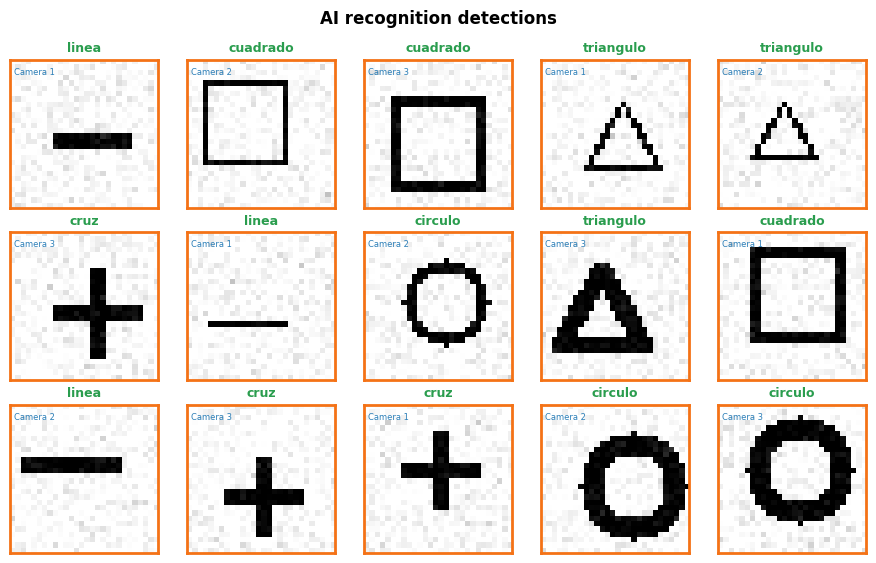
\includegraphics[width=0.85\textwidth]{../img/hoja_detecciones.png}
\caption{Detecciones reconocidas por la CNN (etiqueta en verde, c\'amara en azul).}
\label{fig:detecciones}
\end{figure}

\section{Pruebas end-to-end y tolerancia a fallos}\label{sec:e2e}
Levantamos el c\'umulo con los tres nodos (Java + Python + Go) y el Servidor de
Testeo con las 3 c\'amaras. El sistema funciona de punta a punta:

\begin{itemize}[nosep,leftmargin=1.4em]
  \item El c\'umulo heterog\'eneo \textbf{elige l\'ider} sin intervenci\'on.
  \item La CNN \textbf{reconoce en las 3 c\'amaras} en paralelo (un hilo por
        c\'amara), con \textbf{88--100\% de acierto} por c\'amara.
  \item Los tres nodos aplican las \textbf{mismas 75 detecciones en el mismo
        orden}: el registro queda id\'entico en Java, Python y Go.
\end{itemize}

\paragraph{Consistencia del registro.} La forma de verificar que la r\'eplica
qued\'o bien fue comparar el registro de los tres nodos al final de la corrida:
pedimos \texttt{LEER\_REGISTRO} a cada uno y comparamos las 75 detecciones. Las
tres respuestas \texttt{REGISTRO|...} salieron id\'enticas, con las detecciones
en el mismo orden. Esto confirma que Raft no solo replic\'o el contenido, sino
tambi\'en el orden, que es lo que garantiza la m\'aquina de estado
determinista: aplicar el mismo log en el mismo orden lleva a los tres nodos al
mismo estado.

\paragraph{Failover.} Para probar tolerancia a fallos matamos al l\'ider mientras
el sistema segu\'ia insertando. En esa corrida el l\'ider era el nodo Python. Al
caer, los seguidores dejan de recibir latidos, salta el timeout de elecci\'on y
\textbf{Go es reelegido l\'ider en el siguiente \emph{term}}. El registro
sobrevive consistente (ninguna detecci\'on committed se pierde) y se sigue
insertando con normalidad. Esto ejercita justo la parte dif\'icil de Raft: cambiar
de l\'ider sin corromper ni reordenar el log ya confirmado.

% TODO: reemplazar este hueco por el screenshot real del Cliente Vigilante en vivo.
\begin{figure}[h]\centering
\fbox{\parbox[c][4.5cm][c]{0.8\textwidth}{\centering\color{cgray}
  \texttt{[ Screenshot del Cliente Vigilante en vivo ]}\\[4pt]
  \scriptsize (pendiente de capturar: ventana del Cliente Vigilante mostrando el
  registro replicado en tiempo real)}}
\caption{Cliente Vigilante mostrando el registro replicado (captura pendiente).}
\label{fig:vigilante}
\end{figure}

\section{C\'omo ejecutar}
Todo es local, sin internet. Se entrena la CNN una vez para generar los pesos
\texttt{.npz}; luego se levantan los tres nodos Raft (cada uno en su lenguaje) y
por \'ultimo el Servidor de Testeo y el Cliente Vigilante.

\begin{enumerate}[nosep,leftmargin=1.5em]
  \item Entrenar la CNN (Python + NumPy) $\to$ guarda pesos en \texttt{.npz}.
  \item Arrancar los 3 nodos Raft: Java, Python y Go, cada uno con su puerto.
        Escuchan en \texttt{0.0.0.0}, as\'i que sirven tanto en localhost como en
        LAN/WIFI.
  \item Arrancar el Servidor de Testeo (Python), que carga los pesos y abre un
        hilo por c\'amara.
  \item Arrancar el Cliente Vigilante (Java) para ver el registro replicado.
\end{enumerate}

\section{Conclusiones y trabajo futuro}
\begin{itemize}[nosep,leftmargin=1.4em]
  \item Armamos un c\'umulo \textbf{poliglota} (Java + Python + Go) donde los tres
        nodos corren su propia implementaci\'on de \textbf{Raft a mano} sobre TCP
        crudo, cumpliendo la restricci\'on de no usar frameworks ni MQ.
  \item La \textbf{CNN desde cero en NumPy} clasifica las 5 figuras con 97.2\% en
        test, y su \textbf{entrenamiento distribuido} baja el tiempo de 11.0\,s a
        4.7\,s con 4 workers sin perder accuracy.
  \item El sistema es consistente de punta a punta: 75 detecciones aplicadas en
        el mismo orden por los tres nodos, y \textbf{failover} verificado (muere
        el l\'ider Python, Go es reelegido, el registro sobrevive).
  \item \textbf{Trabajo futuro / despliegue f\'isico:} correr los nodos en varias
        PCs sobre LAN/WIFI y en 2 sistemas operativos distintos. El c\'odigo ya
        escucha en \texttt{0.0.0.0}, as\'i que la demo multi-PC es cuesti\'on de
        levantar cada nodo en su m\'aquina; falta la corrida f\'isica en clase.
\end{itemize}

\end{document}
